\chapter{Rendering Mode 1}
Erklärung des Mode 1 Renderings am Beispiel \textbf{sbb\_aff.gba} vom \textbf{Tonc\_code}. Es wird lediglich auf einen Teil des Beispielcodes eingegangen, da ein vollständige Erklärung den Rahmen dieser Arbeit sprengen würden.
Im Mode 1 hat der GBA nicht nur reguläre Backgrounds, sondern auch einen affinen Background. 
Dieser affine Background ermöglicht es, eine geometrische Transformation um einen Punkt zu erreichen. Dies sind unter anderem eine Skalierung und/oder ein Rotation des Hintergrundes. Diese speziellen Hintergründe können, je nach Einstellung im Code verschiedene Größen vorweisen, welche über \textbf{DEFINES} vorgegeben sind. Folgende Tabelle soll dies veranschaulichen:
\begin{table}[ht]
\centering
\begin{tabular}{|c|c|c|c|}
\hline
\textbf{Size} & \textbf{Define} & \textbf{Tiles} & \textbf{Pixels} \\ \hline
00 & BG\_AFF\_16x16 & 16x16 & 128x128 \\ \hline
01 & BG\_AFF\_32x32 & 32x32 & 256x256 \\ \hline
10 & BG\_AFF\_64x64 & 64x64 & 512x512 \\ \hline
11 & BG\_AFF\_128x128 & 128x128 & 1024x1024 \\ \hline
\end{tabular}
\caption{Einstellungen des affinen Hintergrundes}
\label{size}
\end{table}


\section{Affine Background Control Register}
Das primäre Register, welchen den Hintergrund identifiziert, hat die Definition REG\_BGxCNT. Das \textbf{X} ist ein Platzhalter für den Hintergrund, der angesprochen wird. Im Mode 1 wäre das \textbf{REG\_BG2CNT} der skalierbare Hintergrund 2. Dieses Register hat die Länge zwei und die Adresse \textbf{ 0400:0008h + 2*x} . Das Register hat folgende Spezifikationen:
\begin{table}[ht]
\centering
\begin{tabular}{|c|c|c|c|c|c|c|c|}
\hline
\textbf{F E} & \textbf{D} & \textbf{C B A 9 8} & \textbf{7} & \textbf{6} & \textbf{5 4} & \textbf{3 2} & \textbf{1 0} \\ \hline
Sz & Wr & SBB & CM & Mos & - & CBB & Pr \\ \hline
\end{tabular}
\caption{REG\_BGxCNT Spezifikationen}
\label{regspec}
\end{table}

\newpage

\begin{table}[h!]
\centering
\begin{tabular}{|p{1cm}|p{1cm}|p{4cm}|p{9cm}|}
\hline
\textbf{Bits} & \textbf{Name} & \textbf{Definition} & \textbf{Beschreibung} \\ \hline
0 - 1 & Pr & BG\_PRIO\# & \textbf{Priority}: Legt die Reihenfolge für das Zeichnen der Hintergründe fest \\ \hline
2 - 3 & CBB & BG\_CBB\# & \textbf{Character Base Block}: Setzt den Charblock der als Basis für den Index der Tiles dient. Mögliche Werte 0 - 3 \\ \hline
6 & Mos & BG\_MOSAIC & \textbf{Mosaic}: Aktiviert den Mosaic Effekt \\ \hline
7 & CM & \begin{tabular}[c]{@{}l@{}}BG\_4BPP,\\ BG\_8PP\end{tabular} & \textbf{Color Mode}: zu Deutsch Farbmodus. Wenn das Bit gesetzt ist, dann 256 Farben, wenn nicht gesetzt, dann 16 verschiedene Farben \\ \hline
8 - C & SBB & BG\_SBB\# & \textbf{Screen Base Block}: Setzt den Bildschirmblock der als Basis für den Index der Map/Karte dient. Mögliche Werte 0 - 31 \\ \hline
D & Wr & BG\_WRAP & \textbf{Affine Wrapping}: Falls gesetzt, dann rotieren die affinen Hintergründe um ihre Kanten. Diese Einstellung hat jedoch keine Auswirkung auf reguläre Hintergründe \\ \hline
E - F & Sz & BG\_SIZE & \textbf{Background Size}: hier wird die Hintergrundgröße eingestellt. \\ \hline
\end{tabular}
\caption{REG\_BGxCNT Detailbeschreibung}
\label{regspecdetail}
\end{table}

Um die Tabelle näher zu erläutern, wird in einem Beispiel der Wert \textbf{BG\_WRAP} gesetzt und danach beschrieben, welche Auswirkung dies hat. Der Background 2, welche für die Darstellung der skalierbaren Kacheln zuständig ist, hat den kompletten Bildschirm des mGBA eingenommen. Lässt man den Wert weg, sieht man wieder einen schwarzen Hintergrund. Mit \textbf{BG\_WRAP} ist dies nicht mehr möglich, weil der Hintergrund dann die Kacheln sind. Man kann dies mit einem Desktophintergrund vergleichen, welcher den kompletten Bildschirm belegt. 
Bemerkung: BG\_WRAP ist nur bei rotier- und skalierbaren Hintergründen möglich. Bei regulären Hintergründen funktioniert diese Einstellung nicht!

\section{init\_map() Funktion}
In diesem Abschnitt wird die \textbf{init\_map()} Funktion nähert behandelt, welche für das Initialisieren und dem Zeichnen der Kacheln zuständig ist. \\
Zuerst das Code Snippet:

\lstinputlisting[language=C, frame=single, breaklines = true, numbers=left, basicstyle=\ttfamily, keywordstyle=\color{blue}\ttfamily, stringstyle=\color{red}\ttfamily, commentstyle=\color{green}\ttfamily, label=initmap,caption=init\_map() Funktion]{code/initmap.c}

Die Variable \textbf{ses} ist der Platzhalter für die Beschreibung der Farben der jeweiligen Tiles, die dann angezeigt werden. In der folgenden Tabelle wird das Farbspektrum und die Ausgabe der Farben näher beschrieben. Dies ist für das Verständnis wichtig, wie der mGBA die Farben berechnet und ausgibt. In diesem Standardbeispiel sind es acht verschieden Farben die jeweils immer über vier Spalten und Zeilen gemeinsam ausgegeben werden. Da die Iteration über 16 Werte geht, wird ab Wert 0x08 wieder die gleiche Farbe, wie bei 0x01 angezeigt.

\begin{table}[h]
\centering
\resizebox{\textwidth}{!}{%
\begin{tabular}{|l|l|l|l|l|l|l|l|l|}
\hline
\textbf{Hex}   & \begin{tabular}[c]{@{}l@{}}0x1, \\ 0x9\end{tabular}               & \begin{tabular}[c]{@{}l@{}}0x2, \\ 0xA\end{tabular}                & \begin{tabular}[c]{@{}l@{}}0x3, \\ 0xB\end{tabular}                & \begin{tabular}[c]{@{}l@{}}0x4, \\ 0xC\end{tabular}                & \begin{tabular}[c]{@{}l@{}}0x5, \\ 0xD\end{tabular}               & \begin{tabular}[c]{@{}l@{}}0x6, \\ 0xE\end{tabular}                  & \begin{tabular}[c]{@{}l@{}}0x7, \\ 0xF\end{tabular}                 & \begin{tabular}[c]{@{}l@{}}0x8, \\ 0x10\end{tabular}                 \\ \hline
\textbf{Farbe} & \begin{tabular}[c]{@{}l@{}}Rot mit \\ grauen Schrift\end{tabular} & \begin{tabular}[c]{@{}l@{}}Grün mit \\ pinker Schrift\end{tabular} & \begin{tabular}[c]{@{}l@{}}Geld mit \\ blauer Schrift\end{tabular} & \begin{tabular}[c]{@{}l@{}}Blau mit \\ gelber Schrift\end{tabular} & \begin{tabular}[c]{@{}l@{}}Pink mit \\ grüner Schrit\end{tabular} & \begin{tabular}[c]{@{}l@{}}Bläulich mit\\ roter Schrift\end{tabular} & \begin{tabular}[c]{@{}l@{}}Weiß mit \\ oranger Schrift\end{tabular} & \begin{tabular}[c]{@{}l@{}}Orange mit \\ weißer Schrift\end{tabular} \\ \hline
\end{tabular}%
}
\caption{Farbdarstellung der Tiles}
\label{tilesfarbe}
\end{table}

\begin{wrapfigure}{r}{0mm}
	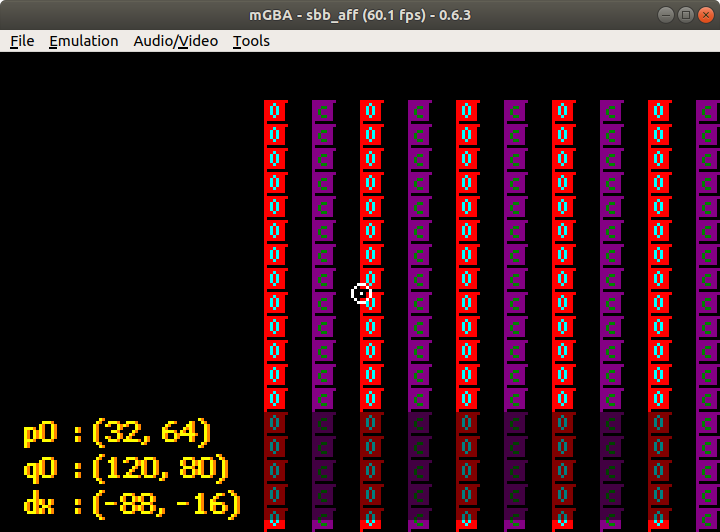
\includegraphics[height=50mm]{img/gerade.png}
	\caption{Anzeige der geraden Kacheln}
	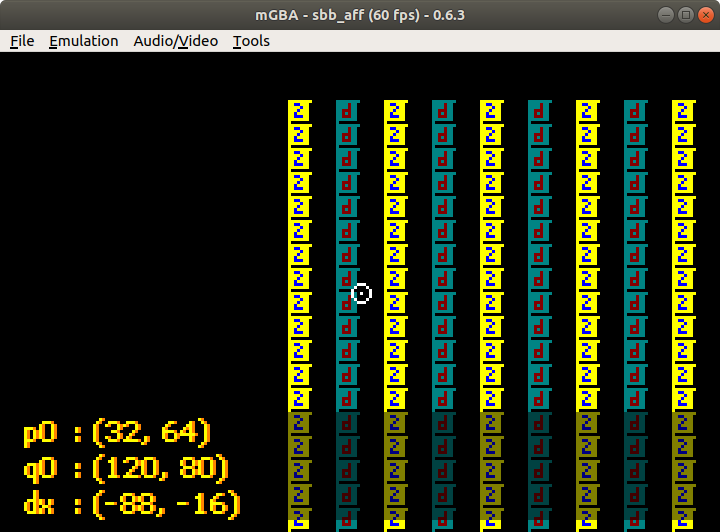
\includegraphics[height=50mm]{img/ungerade.png}
	\caption{Anzeige der ungeraden Kacheln}
\end{wrapfigure}
Der achtstellige Hexadezimalwert von der Variable ses lässt sich in vier Kategorien einteilen, die dann die jeweiligen Spalten darstellen
Als Beispiel hierfür, werden einmal die geraden Spalten und die ungeraden Spalten mit unterschiedlichen Farben angezeigt. 
An diesen beiden Bilder erkennt man, dass einmal die geraden Spalten mit rot und und pink belegt sind und die ungeraden mit gelb und bläulicher Farbe. Dies kann man den Hexwerten von \textbf{ses = 0x000D0001} entnehmen. Die letzte eins entspricht der ersten Spalte bei der Anzeige. Beim unteren Bild erkennt man schön den Spaltenversatz zum obigen Bild. Das resultiert daraus, dass hier nur die ungeraden Spalten angesprochen werden. Der Hexadezimalwert ist im unteren Beispiel mit dem Wert \textbf{ses = 0x0E000300} versehen. Diese Beispiel zeigt, dass man in der Lage ist, die einzelne Spalten beliebig farblich zu verändern und anzupassen. Darüber hinaus sieht man im Code - Snippet \textbf{ses += 0x0000000}. Hier können die Farben auch angepasst werden, nur dass die sich dann Zeilenweise verändern. Zum Beispiel ist es dabei möglich zwei Zeilen mit rot zu belegen, danach dann zwei Zeilen mit einer anderen Farbe. Man hat auch die möglichkeit vier Zeilen mit einer anderen Farbe zu belegen oder jede Zeile.Dies ist abhängig anhander der Einstellung die man wählt. Hier spielt dann die Variable \textbf{pse += MAP\_AFF\_SIZE/4} eine nützliche Rolle. Bei /4 werden vier Zeilen jeweils mit der gleichen Farbe angezeigt. Bei /8 werden lediglich nur zwei Zeilen mit der gleichen Farbe versehen.

\section{Skalierbare und rotierbarer Hintergrund}
Die Funktion sbb\_aff() übernimmt die komplette Aufgabe bezüglich Rotierbarkeit und Skalierung der Tiles, welche von der Funktion init\_map() gezeichnet werden. Im Folgenden wird auf die Funktion sbb\_aff() näher eingegangen und diese ausführlich erläutert. Die Funktion übernimmt unter anderem das Zeichen der $p_{0}$, $q_{0}$ und dx Variablen beziehungsweise Koordinanten, welche im mGBA unten rechts angezeigt werden. Hier wird lediglich eine print-Funktion aufgerufen, welche die aktuellen Werte ausliest und eine Ausgabe ermöglicht. Die print-Funktion wird hier nicht näher erläutert, sondern die Konzentration liegt bei der Skalierung und Rotierbarkeit der Karte. Die affinen Tilemaps benutzen andere Register, welche für diese Dynamik ausgelegt sind. Anstatt \textbf{REG\_BGxHOFS} und \textbf{REG\_BGxVOFS} benutzen die affinen Hintergründe die Register \textbf{REG\_BGx}X und \textbf{REG\_BGxY,} wobei hier \textbf{x} für den Hintergrund steht. Im folgenden wird näher auf die Register und auf die Transformation der affinen Hintergründe eingegangen. Es werden auch anschaulich die mathematischen Operationen aufgezeigt. Die Register sind in zwei unterschiedliche Typen aufgeteilt. Das eine ist für den Vektor dx (\textbf{REG\_BGxX} und \textbf{REG\_BGxY}) zuständig, das andere für die affine \textit{Matrix P} (\textbf{REG\_BGxPA} und \textbf{REG\_BGxPG}) zuständig. Auf die Matrix P wird aufgrund des Umfanges nicht näher darauf eingegangen.
\begin{table}[h]
\centering
\begin{tabular}{|c|c|c|}
\hline
\textbf{Register}                                                & \textbf{Länge} & \textbf{Adresse}      \\ \hline
REG\_BGxCNT                                                      & 2              & 0400:0008h + 2*x      \\ \hline
\begin{tabular}[c]{@{}c@{}}REG\_BGxPA,\\ REG\_BGxPD\end{tabular} & 2              & 0400:0020h + 10*(x-2) \\ \hline
REG\_BGxX                                                        & 4              & 0400:0028h + 10*(x-2) \\ \hline
REG\_BGxY                                                        & 4              & 0400:002Ch + 10*(x-2) \\ \hline
\end{tabular}
\caption{Register der affinen Hintergruende}
\label{affineregister}
\end{table}


\subsection{Transformation der Tilemap}
Die Variable dx beinhaltet die Hintergrundkoordinaten zum Zeitpunkt der Initialisierung der Map.
Die Matrix P beschreibt die Transformation (Rotierung) der X und Y Koordinaten der Map. Dies ist wie folgt mathematisch definiert:
\begin{equation}
T(dx)p := p + dx
\end{equation}
\begin{equation}
T^{-1}dx = T(-dx)
\end{equation}
\begin{equation}
P = A^{-1}
\end{equation}
\begin{equation}
T(dx)q = p
\end{equation}
\begin{equation}
P * q = p
\end{equation}
\begin{equation}
q = A * T(-dx)p
\end{equation}
\begin{equation}
T(dx)P * q = p
\end{equation}
\begin{equation}
P * (q-q_{0}) = (p-p_{0})
\end{equation}
\begin{equation}
dx + P * q_{0} = p_{0}
\end{equation}
\begin{equation}
dx = p_{0} - P * q_{0}
\end{equation}
\begin{table}[h]
\centering
\begin{tabular}{|l|l|}
\hline
p  & Punkt in der X-Koordinate                             \\ \hline
q  & Punkt in der Y-Koordinate                             \\ \hline
dx & Vector für die Verschiebung (REG\_BGxX und REG\_BGxY) \\ \hline
A  & Transformation von X zu Y Koordinate                  \\ \hline
P  & Transformation von Y zu X Koordinate                  \\ \hline
\end{tabular}
\caption{Erlaeuterung der mathematischen Varbiablen}
\label{mathavar}
\end{table}
\newpage
Wenn der Verschiebungsvektor dx verwendet wird, dann wird eine Transformation um den Punkt $p_{0}$gemacht. Das führt zu der y-Punktkoordinate $q_{0}$im Bild. Die Multiplikation $p_{0}* P$ ist die Korrektur der X-Koordinate. Dies ist notwendig, um die Rotation um den Punkt $q_{0}$, anstatt um (0,0) zu ermöglichen. Im Beispiel sbb\_aff.c wird diese Transformation von der Funktion \textbf{bg\_rotscale\_ex()} übernommen.
\begin{figure}[h]
	\centering
	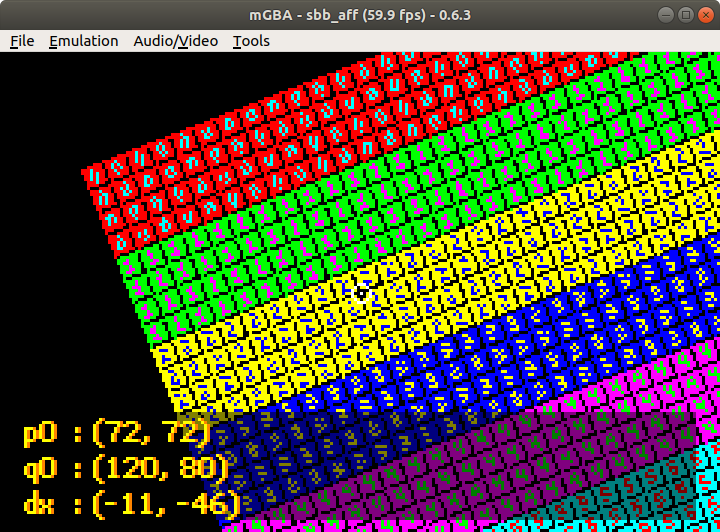
\includegraphics[height=85mm]{img/rotation.png}
	\caption{Rotationbeispiel der Tiles}
\end{figure}

Hier ist das Code-Snippet mit eingefügten Kommentaren, um die Verständnis des Codes zu erleichtern. Die Kommentare sind ergänzt und der Quellcode ist ausführlich mit dem mGBA getestet worden. Auch hier würde eine detailiertere Beschreibung den Rahmen dieser Studienarbeit sprengen.
\lstinputlisting[language=C, breaklines = true, numbers=left, frame=single, basicstyle=\ttfamily, keywordstyle=\color{blue}\ttfamily, stringstyle=\color{red}\ttfamily, commentstyle=\color{green}\ttfamily, label=sbbaff,caption=sbb\_aff() Funktion]{code/rotate.c}
